\section{State of the art}

\subsection{Taxonomy}

It is certainly useful to start with a review of the different ways to categorize the features and algorithms used by researchers in the field. The goal is to define our needs precisely and select the important things to consider.

\subsubsection{Taxonomy for features} \label{features_tax}

The features we select must allow us to identify a precise device among potentially very similar devices. We need what \textcite{delgado_passive_2020} describe as a Physical Unclonable Function (PUF). PUFs are physical distortions that are unique to a specific system. They are another way of talking about fingerprints.

\textcite{xu_device_2015} propose three ways to categorize radio signal features:

\begin{itemize}
  \item based on the specificity of the feature (from vendor specific to device specific),
  \item based on the layers (PHY, MAC, Network and higher),
  \item and based on the acquisition method (passive or active).
\end{itemize}

Whether we end up with a system that is able to identify many devices uniquely, or one that only tries to separate a specific device from the others, we will need device specific accuracy. We don't want to make relay attacks impossible only if the attacker doesn't use a device from the same vendor as the victim's device.

Features from the MAC and higher layers typically require in depth knowledge of the protocols in play. Not only that, but they also tend to be less specific than we would like (either vendor specific or depending on the type of device). This indicates we should probably focus on the physical (PHY) layer features, which rely on imperfections in the manufacturing process of the devices.

\subsubsection{Taxonomy for fingerprinting algorithms}

\textcite{riyaz_deep_2018} provide a visual categorization of fingerprinting approaches, which we adapt in figure \ref{fig:algo-taxo}. We take a look at these approaches in the following paragraphs.

\begin{figure}[htp!]
  \centering
  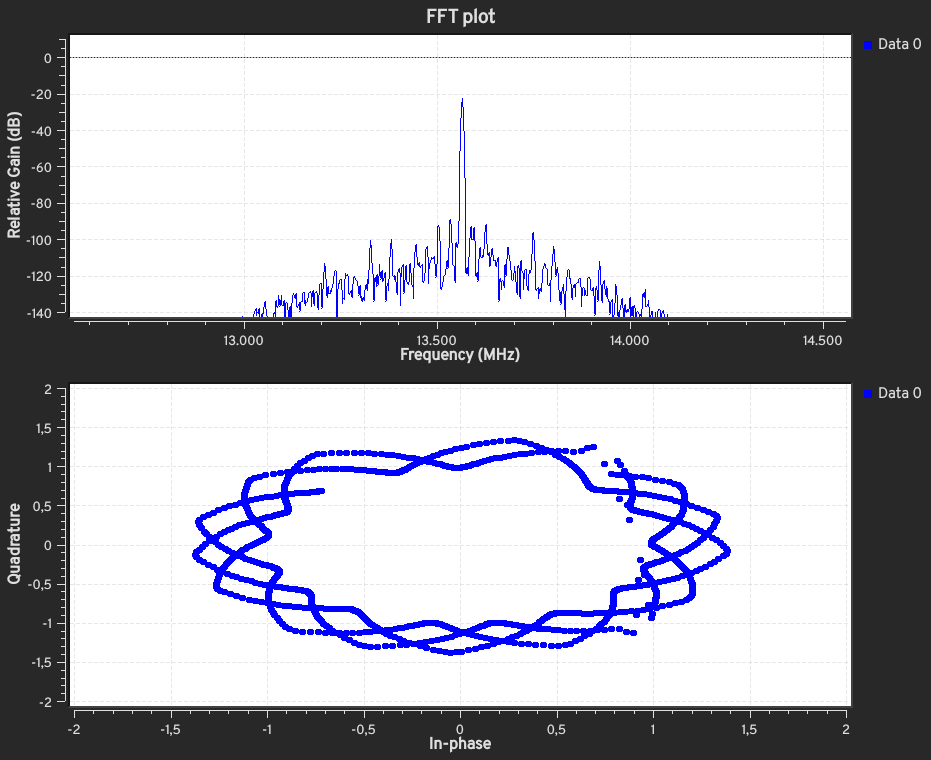
\includegraphics[scale=0.3]{figures/grc_transient-flower.png}
  \caption{Fingerprinting algorithms taxonomy}
  \label{fig:algo-taxo}
\end{figure}

\paragraph{Supervised approaches:} Supervised approaches use features from labelled data to generate a function capable of separating the different classes. These approaches can be further categorized in similarity based and classification techniques.

Similarity based techniques are white-list algorithm that use a database of fingerprints and a similarity measure to determine whether a device is legitimate. Developing a technique like this requires prior knowledge of vendor specific device features \cite{riyaz_deep_2018}. Classification systems can also require deep knowledge of the features and protocols used, in the case of "traditional", manually tuned classifiers. Those are built to extract predetermined features and work similarly to other white-list algorithms afterwards.

The classification algorithms we are most interested in are deep learning techniques, which are able to extract the features they need by themselves. This can be done through deep Multi-Layer Perceptrons (MLP) \cite{delgado_passive_2020, stankowicz_complex_2019} or through more advanced techniques like Convolutional Neural Networks (CNN) \cite{riyaz_deep_2018, oyedare_estimating_2019, youssef_machine_2017, morin_transmitter_2019, sankhe_no_2019}. The latter have proved very powerful in domains like computer vision, natural language processing and recommendation systems. This success is one of the reasons experimentations on CNNs are common in RFML research.

\paragraph{Unsupervised systems:} Unsupervised approaches cannot by themselves discriminate a legitimate device from an illegitimate one. They don't have that information, since they work with unlabeled data. In order to detect attempts of impersonation, such a system has to keep a record of fingerprints and linked identifiers. It can then throw an alert when multiple fingerprints are linked to the same MAC address or when multiple MAC addresses are linked to the same fingerprint.

\textcite{xu_device_2015} specify that unsupervised approaches are appropriate when the fingerprints of legitimate devices are not available. ... are examples of work on such systems.

\subsection{Features selection}

In section \ref{features_tax} we discussed the different types of features that exist in radio signal data. We concluded that the features we are most interested in are from the physical layer.

transient phase

\subsection{Machine learning applied to radio frequency}

Radio Frequency Machine Learning (RFML)...

Difficulties (ref)

\subsubsection{Comparing approaches}

Several articles have compared the performance of different machine learning approaches.

...

\subsubsection{Neural network architecture}

Inputs (windows, sliding?...)
...


What about \parencite[pre][page 2]{youssef_machine_2017}?

I love \footcite[pre][post]{stankowicz_complex_2019}.


- **Waveform domain techniques** [11], [14], [22], [24], [25] consider time and frequency representation as the basic blocks while **modulation domain techniques** [6] represent signals in terms of I/Q samples.
- Waveform domain techniques are more flexible but more complex. Modulation domain techniques are better structured and well-behaved but require knowledge of the respective modulation scheme.
